\documentclass[tikz,border=10pt]{standalone}
\usepackage{tikz}
\usetikzlibrary{arrows.meta,calc,fit,backgrounds}
\usepackage{xcolor}
\renewcommand{\familydefault}{\sfdefault}
\pagecolor{white!8}

% -------------------------
% Parameters
% -------------------------
\newcommand{\NInput}{6}
\newcommand{\NEncoder}{4}
\newcommand{\NLatent}{2}
\newcommand{\NDecoder}{4}
\newcommand{\NOutput}{6}

\newcommand{\XInput}{0}
\newcommand{\XEncoder}{2.6}
\newcommand{\XLatent}{5.0}
\newcommand{\XDecoder}{7.4}
\newcommand{\XOutput}{10.0}

\newcommand{\LayerSep}{1.05}
\newcommand{\NeuronSize}{7.8mm}

% keeps arrow tips slightly off the node border (like the reference)
\newcommand{\CalloutGap}{2.2mm}

% Colours (matching the VAE diagram)
\colorlet{encFill}{green!15!white}
\colorlet{encStroke}{green!55!black}
\colorlet{latentFill}{orange!15!white}
\colorlet{latentStroke}{orange!55!black}
\colorlet{decFill}{blue!10!white}
\colorlet{decStroke}{blue!45!black}
\colorlet{wireColor}{black!35}

% -------------------------
% Helpers
% -------------------------
\newcommand{\PlaceLayer}[5]{%
  % #1 prefix, #2 count, #3 x-position, #4 fill color, #5 stroke color
  \pgfmathsetmacro{\HalfSpan}{(#2-1)/2}
  \foreach \i in {1,...,#2}{%
    \pgfmathsetmacro{\y}{(\HalfSpan-(\i-1))*\LayerSep}
    \node[circle,draw=#5,line width=0.5pt,minimum size=\NeuronSize,inner sep=0pt,fill=#4]
      (#1\i) at (#3,\y) {};
  }%
}

\newcommand{\ConnectLayers}[4]{%
  % #1 left prefix, #2 left count, #3 right prefix, #4 right count
  \foreach \i in {1,...,#2}{%
    \foreach \j in {1,...,#4}{%
      \draw[wireColor,line width=0.3pt] (#1\i) -- (#3\j);
    }%
  }%
}

\begin{document}
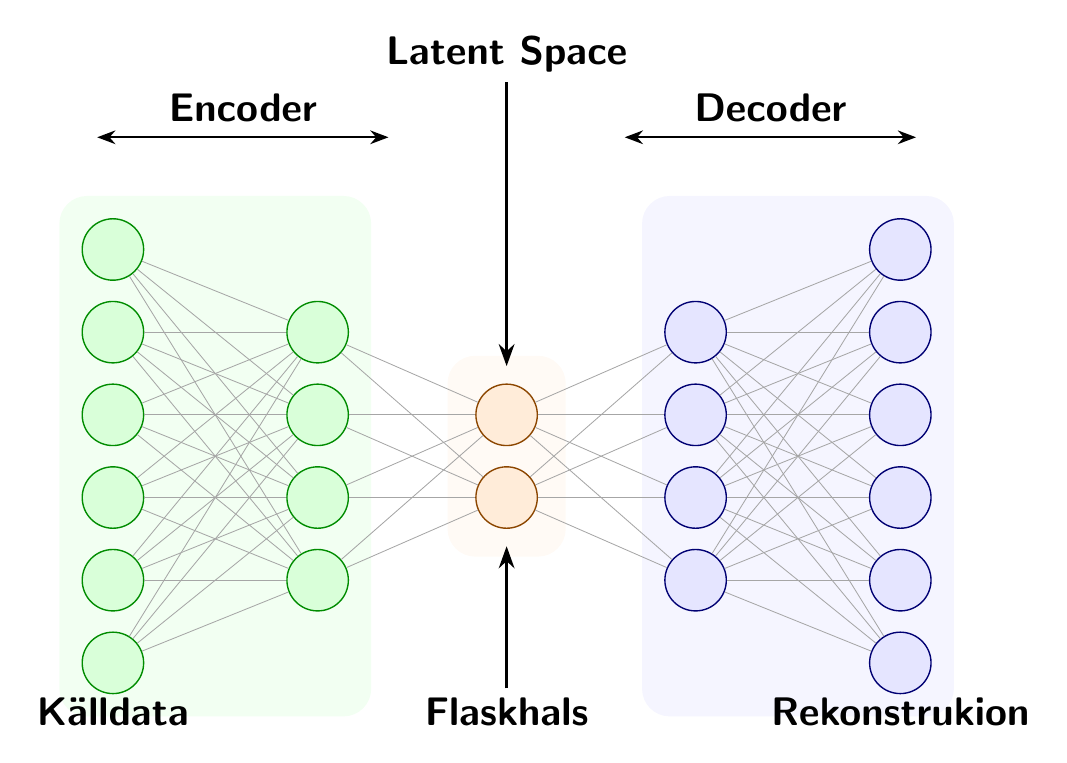
\begin{tikzpicture}[
  >=Stealth,
  title/.style={font=\sffamily\bfseries\Large},
  label/.style={font=\sffamily\bfseries\Large},
  callout/.style={line width=0.95pt,-{Stealth[length=2.8mm,width=2mm]}}
]

% Layers
\PlaceLayer{I}{\NInput}{\XInput}{encFill}{encStroke}
\PlaceLayer{E}{\NEncoder}{\XEncoder}{encFill}{encStroke}
\PlaceLayer{L}{\NLatent}{\XLatent}{latentFill}{latentStroke}
\PlaceLayer{D}{\NDecoder}{\XDecoder}{decFill}{decStroke}
\PlaceLayer{O}{\NOutput}{\XOutput}{decFill}{decStroke}

% Connections
\ConnectLayers{I}{\NInput}{E}{\NEncoder}
\ConnectLayers{E}{\NEncoder}{L}{\NLatent}
\ConnectLayers{L}{\NLatent}{D}{\NDecoder}
\ConnectLayers{D}{\NDecoder}{O}{\NOutput}

% Top arrows/labels
\draw[<->,line width=0.8pt]
  (\XInput-0.2,4.05) -- node[above=2pt,title]{Encoder} (\XEncoder+0.9,4.05);
\draw[<->,line width=0.8pt]
  (\XDecoder-0.9,4.05) -- node[above=2pt,title]{Decoder} (\XOutput+0.2,4.05);

% Latent space callout: ONLY to the outer/top latent node (L1)
\node[title] (latenttitle) at (\XLatent,5.1) {Latent Space};
\draw[callout] (latenttitle.south) -- ($(L1.north)+(0,\CalloutGap)$);

% Bottom labels
\node[label] at (\XInput,-3.25) {Källdata};
\node[label] at (\XOutput,-3.25) {Rekonstrukion};

% Encoded data callout: ONLY to the outer/bottom latent node (L2)
\node[label] (encodedlabel) at (\XLatent,-3.25) {Flaskhals};
\draw[callout] (encodedlabel.north) -- ($(L2.south)+(0,-\CalloutGap)$);

% -------------------------
% Background regions
% -------------------------
\begin{pgfonlayer}{background}
  \node[rounded corners=10pt, fill=green!5, inner sep=8pt,
        fit=(I1)(I\NInput)(E1)(E\NEncoder)] {};
  \node[rounded corners=10pt, fill=orange!4, inner sep=10pt,
        fit=(L1)(L\NLatent)] {};
  \node[rounded corners=10pt, fill=blue!4, inner sep=8pt,
        fit=(D1)(D\NDecoder)(O1)(O\NOutput)] {};
\end{pgfonlayer}

\end{tikzpicture}
\end{document}